\documentclass{report}

\usepackage[T1]{fontenc}
\usepackage[french]{babel}

\spaceskip=2\fontdimen2\font plus 2\fontdimen3\font minus 2\fontdimen4\font
\usepackage{adjustbox}
\usepackage{enumitem}
\usepackage{hyperref}
\usepackage{xcolor}

\hypersetup{
  colorlinks=true,  % Activer la coloration des liens
  linkcolor=blue!80!black,  % Couleur des liens vers d'autres parties du document (table des matières, références)
  citecolor=red,  % Couleur des liens de citation
  urlcolor=blue,    % Couleur des liens URL
  linkbordercolor={0 0 0},  % Couleur de la bordure des liens (noir)
  urlbordercolor={1 1 1},   % Couleur de la bordure des liens URL (blanc)
  citebordercolor={1 1 1}   % Couleur de la bordure des liens de citation (blanc)
}

\usepackage{csquotes}
\usepackage[style=numeric, backend=biber]{biblatex} % Spécifiez le style et le backend
\addbibresource{bibfile.bib} % Chemin vers votre fichier .bib
 
\setcounter{tocdepth}{3}
\usepackage{lipsum} % For generating placeholder text
\usepackage{graphicx} % for including images
\usepackage[a4paper,
            top = 2.5cm,
            bottom = 3 cm,
            left = 2.1 cm,
            right = 2.4 cm]{geometry} % for setting page margins
\usepackage{indentfirst} % for indenting the first paragraph
\usepackage{glossaries} % list des abréviations
\usepackage{float} % for controlling the position of objects
\setlength\parindent{0pt} % for indenting the begining of the paragraph
% Numbering format
\renewcommand{\thesection}{\arabic{chapter}.\arabic{section}}
% \renewcommand{\thesubsection}{\arabic{chapter}.\arabic{section}.\arabic{subsection}}

\begin{document}

\begin{titlepage}

	\begin{center}
		
\includegraphics[width=4.3cm]{logo/ufr.png} % Replace with the filename or path to your left logo
		\hfill
		
\includegraphics[width=6cm]{logo/ueve.png} % Replace with the filename or path to your right logo
		\hfill
		
\includegraphics[width=4cm]{logo/cfa.png} % Replace with the filename or path to your right logo

		\vspace{3cm}
        \newcommand\titleofdoc{\bfseries Rapport de stage }
        \Huge{\titleofdoc} 

        \vspace{0.5cm}
        {\fontsize{15}{20}\textbf{ Mention: E3A}} \\      
        
        {\fontsize{15}{20}\textbf{Parcours : M2 Réalité Virtuelle et Systèmes Intelligents}}\\       

        \vspace{1 cm}

        \LARGE{ Analyse de la saillance et application à la détection et la classification d'images}\\
        \vspace{1 cm}
        {
\includegraphics[width=0.45\textwidth]{logo/tsp.png}}\quad\\
        \vspace{2 cm}
        % \Large{\GroupName}
        \vspace{0.25cm}
        {\bf {EL MHAMDI EL ALAOUI Abdellah}} \\
        Stage effectué du 01/04/2023 au 29/09/2023\\
        \vspace{3 cm}

        \leftline{\fontsize{15}{12}\selectfont \textbf{Tuteur entreprise :}  M. Patrick Horain}
        \leftline{\fontsize{15}{12}\selectfont \textbf{Tuteur pédagogique :} M. Hicham Hadj Abdelkader}
        \vspace{1 cm}         
	\end{center}
\end{titlepage}

\clearpage
\mbox{} % Insère un espace invisible pour forcer la création d'une nouvelle page

% Contenu de la page blanche

\newpage
\chapter*{Remerciements}
\fontsize{12}{17}\selectfont{
\hspace{1.6cm}Je tiens à exprimer ma gratitude envers toutes les personnes qui ont contribué, de près ou de loin, au succès de mon stage et qui m'ont apporté leur soutien dans la rédaction de ce rapport.
\vspace*{2\baselineskip}

\hspace{1.6cm}En tout premier lieu, je souhaite adresser mes remerciements à mon tuteur de stage, Monsieur Patrick Horain de l'école Télécom SudParis, pour sa confiance, sa convivialité et les connaissances précieuses qu'il a partagées avec moi.
\vspace*{2\baselineskip}

\hspace{1.6cm}Je tiens également à adresser mes sincères remerciements aux professeurs de l'Université d'Evry Val d'Essonne pour avoir mis à ma disposition les outils nécessaires à la réussite de mon stage.
\vspace*{2\baselineskip}

\hspace{1.6cm}Un grand merci s'adresse également à toute l'équipe du département Artemis ainsi qu'au personnel de l'école TSP pour leur accueil chaleureux au sein de l'entreprise. Leur amabilité et le temps qu'ils ont généreusement consacré à répondre à mes questions ont grandement contribué à mon expérience.
\vspace*{2\baselineskip}

\hspace{1.6cm}Enfin, je souhaite exprimer ma profonde gratitude envers mes parents, mon frère, ma sœur et mes amis. Leur soutien moral et financier constant, ainsi que leurs conseils avisés, ont été des éléments essentiels tout au long de mon parcours scolaire.
}
\fontsize{12}{12.5}\selectfont{

% Table of Contents
\tableofcontents
\clearpage

% Table of Figures
\listoffigures
}

\fontsize{12}{17}\selectfont{

\vspace*{1\baselineskip}





\chapter{Introduction}
  
\hspace{1.6cm} Les avancées en matière d'intelligence artificielle (IA) ont permis des progrès significatifs dans le domaine de la vision par ordinateur, notamment dans des tâches telles que la classification d'images. Cependant, les résultats obtenus restent souvent difficilement explicables. En particulier, l'activation des réseaux convolutifs est parfois très éloignée de la localisation véritable des objets détectés dans les images.  Cette limitation est particulièrement préoccupante dans des domaines sensibles tels que la médecine, où il est essentiel de pouvoir avoir confiance en les décisions prises par les applications d'IA.
\vspace*{0.5\baselineskip}

\hspace{1.6cm} Dans le cadre de ce stage, l'objectif est d'explorer des méthodes visant à renforcer la fiabilité des décisions de classification en prenant en compte l'activation des réseaux neuronaux pendant l'apprentissage. L'idée sous-jacente est d'utiliser les informations fournies par ces réseaux pour améliorer l'explicabilité et ainsi la confiance accordée aux résultats obtenus.
\vspace*{1\baselineskip}

\hspace{1.6cm} Le travail de recherche comprendra une comparaison entre les approches traditionnelles basées sur les cartes de saillance, telles que GradCam et ScoreCam. L'évaluation de ces méthodes sera réalisée sur deux ensembles de données distincts. Tout d'abord, une évaluation sera effectuée sur la base de données ImageNet, qui est un référentiel couramment utilisé pour évaluer les performances des modèles de vision par ordinateur. Ensuite, une évaluation spécifique sera réalisée sur des images de frottis sanguins pour la détection des parasites responsables de la paludisme, une maladie grave qui affecte de nombreuses personnes à travers le monde.
\vspace*{1\baselineskip}

\hspace{1.6cm} Les résultats attendus de ce stage sont une meilleure compréhension de l'activation des réseaux neuronaux pendant l'apprentissage et le développement de méthodes plus robustes pour la prise de décisions en utilisant ces informations. L'accent sera mis sur l'utilisation de cartes de saillance pour identifier les régions d'intérêt dans les images, afin d'accroître la confiance dans les résultats de classification obtenus.

\chapter{Présentation de l’établissement d’accueil }
\hspace{1.6cm}Mon stage se déroulait à l'école Télécom SudParis. Fondée en 1979, TSP est une grande école publique d'ingénieurs reconnue au meilleur niveau des sciences et technologies du numérique. La qualité de ses formations est basée sur l’excellence scientifique de son corps professoral et une pédagogie mettant l’accent sur les projets d’équipes, l’innovation de rupture et l’entreprenariat. Dans ce chapitre, je vais vous présenter l'entreprise et son service d'accueil.
\begin{figure}[htbp] 
	\centering
        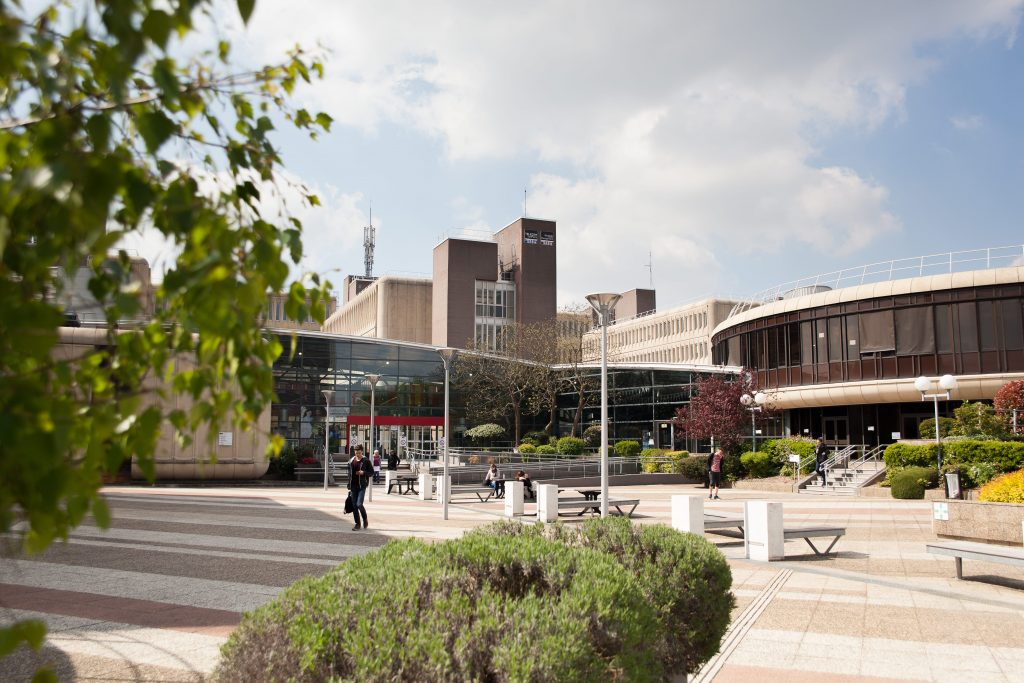
\includegraphics[width=11.5cm]{logo/telecomsudparis.jpg} 
	\caption{Campus de Télécom SudParis}
	\label{fig:Aperçu de Grad-CAM}
\end{figure}
\section{Secteur d'activité }
\hspace{1.6cm} Télécom SudParis est une école d'ingénieurs en télécommunications et technologies de l'information située à Évry, en France. Elle est classée dans le secteur de l'enseignement supérieur et est identifiée par le code APE 8542Z. Ce code APE désigne les établissements d'enseignement supérieur qui proposent des formations dans divers domaines tels que l'informatique, l'électronique, la télécommunication, etc.
\vspace*{0.5\baselineskip}
\newpage

\hspace{1.6cm} En tant qu'école d'ingénieurs spécialisée dans les technologies de l'information et de la communication, Télécom SudParis offre une formation de haut niveau à ses étudiants, qui peuvent se spécialiser dans des domaines tels que la sécurité des réseaux, la communication sans fil, l'intelligence artificielle, etc.

\section{Importance }
\hspace{1.6cm}Télécom SudParis est une école d'ingénieurs à but non lucratif, le chiffre d'affaires n'est pas un indicateur pertinent de son importance. Cependant, l'école emploie environ 200 personnes, dont 103 enseignants-chercheurs permanents. Les autres membres du personnel travaillent dans les services administratifs, les laboratoires de recherche, les centres de formation continue, etc. Télécom SudParis accueille également plus de 2 000 étudiants chaque année, ce qui en fait une institution importante dans le domaine de l'enseignement supérieur en France.
\vspace*{0.5\baselineskip}

\hspace{1.6cm} En outre, l'école TSP fait partie de l'iMT. TSP est l'une des 5 écoles membres de l'Institut Polytechnique de Paris, un groupe d'écoles d'ingénieurs spécialisées dans les technologies de l'information et de la communication, ce qui renforce encore son importance dans le secteur.

\section{Schéma d'organisation succinct}
\hspace{1.6cm} Télécom SudParis est structuré en une Direction, 6 directions métiers, 6 départements d'enseignement et de recherche, 4 services communs avec IMT-BS. Le schéma ci-dessous présente de manière synthétique la structure organisationnelle de Télécom SudParis :
\newpage

% \vspace*{0.5\baselineskip}
\begin{figure}[htbp] % You can adjust the placement options [htbp] as needed
	\centering
        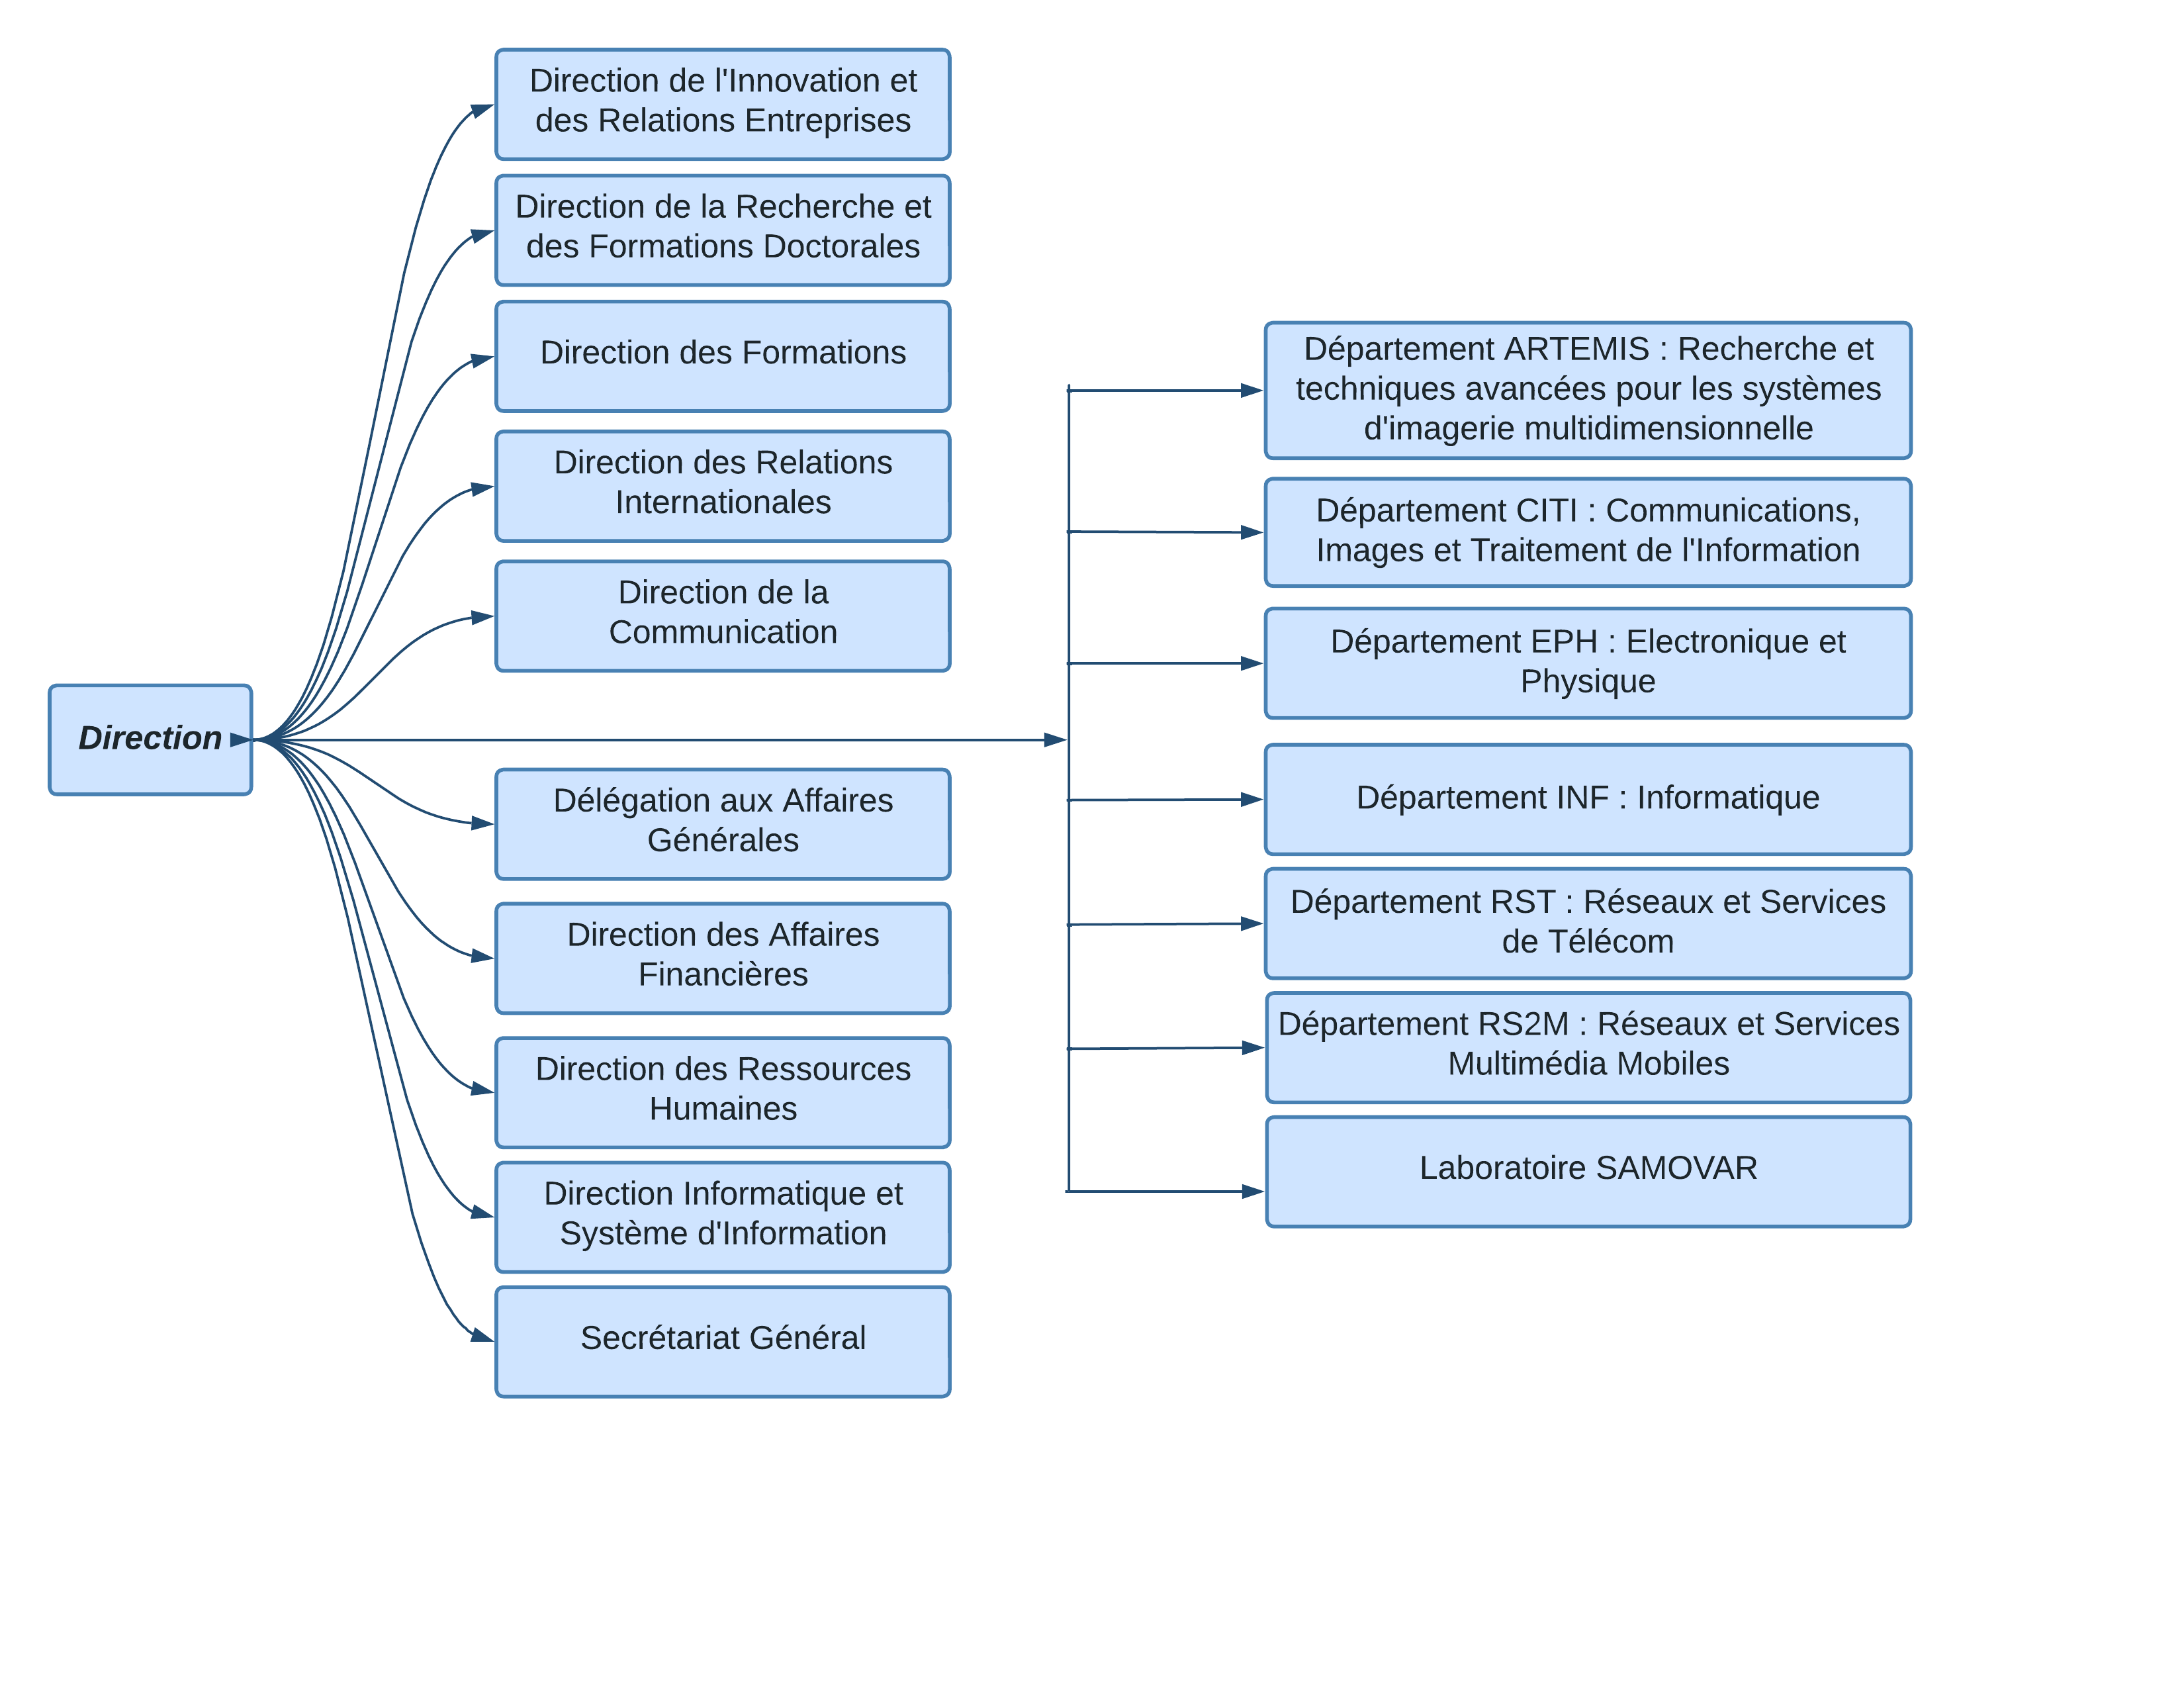
\includegraphics[width=16.5cm]{logo/orga.png} % Replace with the filename or path to your left logo
	\caption{organigramme de Télécom SudParis}
	\label{fig:organigramme de Télécom SudParis}
\end{figure}

\section{Organisation du service}
\hspace{1.6cm} Dans Télécom SudParis, il existe un laboratoire appelé SAMOVAR, qui regroupe plusieurs équipes de chercheurs travaillant dans le domaine des services, des réseaux et des télécommunications. En plus de cela, il y a également différents départements de recherche qui rassemblent des enseignants-chercheurs issus du laboratoire SAMOVAR. J'ai eu l'opportunité d'effectuer mon stage dans le département ARTEMIS.
\subsection{SAMOVAR }
\hspace{1.6cm} Le laboratoire SAMOVAR (Services répartis, Architectures, Modélisation, Validation, Administration des Réseaux) regroupe plusieurs équipes de chercheurs qui travaillent dans le domaine des services, des réseaux et des télécommunications.

\hspace{1.6cm} SAMOVAR est un des rares laboratoires à couvrir l’ensemble des thématiques des systèmes de communications. Menées en relation avec des industriels, ses activités allient qualité scientifique et originalité.

\subsection{ARTEMIS }
\hspace{1.6cm}Le département ARTEMIS a été créé en 1999. Il regroupe aujourd'hui une trentaine de personnes. Le cœur des recherches d'ARTEMIS relève des sciences et technologies de l'image numérique. Celles-ci lancent en effet de nombreux défis aux acteurs économiques et académiques afin de concevoir méthodes innovantes et nouveaux services pour la société de l'information. L'image numérique d'aujourd'hui couvre le large éventail des données visuelles : multimédia (ex : photos, télévision), biologiques (scanner, microscipie...) ou 3D (réalité virtuelle et augmentée...) en environnement fixe ou mobile.
\vspace*{0.5\baselineskip}

\hspace{1.6cm} ARTEMIS traite de la chaîne de l'image depuis la création des contenus numériques jusqu'à leur diffusion. L'enjeu est de créer, modéliser, analyser, indexer, animer, sécuriser, manipuler, enrichir, coder, distribuer et visualiser des contenus hétérogènes et complexes pour des services d'intermédiation économiquement réalistes.

\section{Rôle du tuteur entreprise }
\hspace{1.6cm} Mon tuteur entreprise, Monsieur Patrick Horain est membre du département ARTEMIS à Telecom SudParis. Ses activités d'enseignement consistent à créer des unités de cours et des conférences pour les étudiants en ingénierie et en master. Il coordonne le domaine académique de l'image, du multimédia et des applications à Telecom SudParis.
\vspace*{0.5\baselineskip}

\hspace{1.6cm}Ses intérêts de recherche portent sur le traitement d'images et la vision par ordinateur en général. Il possède une longue expérience dans les interfaces perceptives pour l'interaction homme-machine. Au sein du réseau de recherche du CNRS sur l'Information, le Signal, les Images et la Vision (ISIS), il a coanimé une action spéciale sur le visage, le geste, l'action et le comportement (2009-2016). Il a coorganisé et présidé les conférences internationales IHCI 2014 et IHCI 2017 sur l'interaction homme-machine intelligente. Il a également présidé le comité d'organisation de la conférence Web3D 2022.

\chapter{Contexte de la mission }

\section{Présentation du contexte de la mission}
\hspace{1.4cm}Le paludisme, également connu sous le nom de malaria, est une maladie infectieuse grave transmise par les moustiques et causée par les parasites du genre Plasmodium qui attaquent les globules rouges du sang. Ses symptômes courants tels que la fièvre, les frissons, les maux de tête et les douleurs musculaires nécessitent une détection et un traitement rapides pour éviter des complications graves.
\begin{figure}[htbp] 
	\centering
        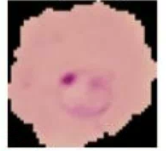
\includegraphics[width=3cm]{logo/Malaria_img_inf.png} 
	\caption{Exemple d'image de cellule infectée}
	\label{fig:Exemple image de cellule infectée}
\end{figure}

\hspace{1.4cm}Traditionnellement, le diagnostic du paludisme se fait par la méthode du frottis sanguin au microscope, mais la détection précise des parasites est un défi en raison de leur variabilité et de leur faible concentration dans le sang. C'est là que les méthodes automatiques, comme l'utilisation d'algorithmes de détection tels que les réseaux de neurones, peuvent apporter une aide précieuse. Ces approches automatisées permettent de traiter de vastes quantités de données et de rechercher des caractéristiques spécifiques des parasites, offrant ainsi une alternative prometteuse pour améliorer la détection précoce et le traitement rapide de cette maladie potentiellement mortelle.
\vspace*{0.5\baselineskip}

\hspace{1.6cm}Cependant, malgré les défis liés à l'interprétation des résultats des algorithmes de détection (notamment les réseaux de neurones), leur utilisation peut apporter des informations précieuses pour orienter les professionnels de la santé dans l'analyse d'échantillons sanguins et dans la prise de décisions cliniques en vue d'un diagnostic plus précis et d'un traitement rapide du paludisme. Il convient de souligner qu'une condition pour établir la santé d'un patient est d'examiner au moins 200 000 globules rouges et de ne pas y détecter de parasites.

\section{Description de la mission }
\hspace{1.4cm}Ce rapport de stage porte sur une mission passionnante réalisée au sein du département ARTEMIS de l'école Telecom SudParis. Notre objectif principal était d'étudier les cartes de saillance dans le domaine de la vision par ordinateur et de trouver des moyens de renforcer la fiabilité des décisions de classification obtenues par les réseaux convolutifs.
\vspace*{0.5\baselineskip}

\hspace{1.6cm}Pour remédier à ce problème, notre objectif principal dans ce stage était d'explorer des approches qui prennent en compte l'activation des cartes de saillance lors de l'apprentissage. Pour évaluer ces approches, nous avons utilisé deux ensembles de données distincts. Tout d'abord, nous avons utilisé la base d'images ImageNet, qui est largement utilisée dans la recherche en vision par ordinateur. Ensuite, nous nous sommes concentrés sur des images de frottis sanguins pour la détection des parasites Plasmodium, responsables du paludisme.
\vspace*{0.5\baselineskip}

\hspace{1.6cm}Une chose à noter est que ce stage fait suite aux travaux réalisés par deux anciens stagiaires. Le premier stagiaire, Adam Allah, a réalisé un état de l'art sur les modèles de classification et les approches de génération des cartes d'activation\cite{Adam21}. Le deuxième stagiaire, Wyctor Fogos da Rochas, a tenté d'entraîner un modèle (VGG16\cite{simonyan2015deep}) en utilisant un entraînement personnalisé pour améliorer les cartes d'activation\cite{Wyctor22}(nous reviendrons sur ces travaux dans les sections suivantes).
\vspace*{0.5\baselineskip}

\hspace{1.6cm}Dans les chapitres qui suivent, nous expliquons les travaux réalisés par Adam et Wyctor. Nous détaillons également les différentes étapes que nous avons suivies tout au long du stage, notamment la collecte des données, la mise en œuvre des modèles de réseaux convolutifs, la génération des cartes de saillance, les expérimentations réalisées et l'évaluation des performances de nos approches. Nous présenterons en détail notre approche, les résultats obtenus et les analyses effectuées.

\section{Problématique}
\hspace{1.6cm}Dans les réseaux de neurones convolutifs (CNN), les activations font référence aux régions spécifiques d'une image qui sont fortement responsables de la décision prise par le modèle. Ces régions sont détectées par le CNN en réponse à des caractéristiques visuelles significatives liées à la classe de l'objet. Cependant, certaines techniques l'explication de la catégorie peuvent parfois donner des résultats incohérents, où les zones activées ne correspondent pas toujours à la véritable région de l'objet de la catégorie prédite. 

Voici deux exemples \ref{fig:Exemples d'Activation : Activation Pertinente et Non Pertinente} d'images correctement classées, accompagnés de leurs activations par rapport à la classe de vérité de terain, illustrant à la fois une activation pertinente et une activation moins précise:

\begin{figure}[htbp] 
	\centering
        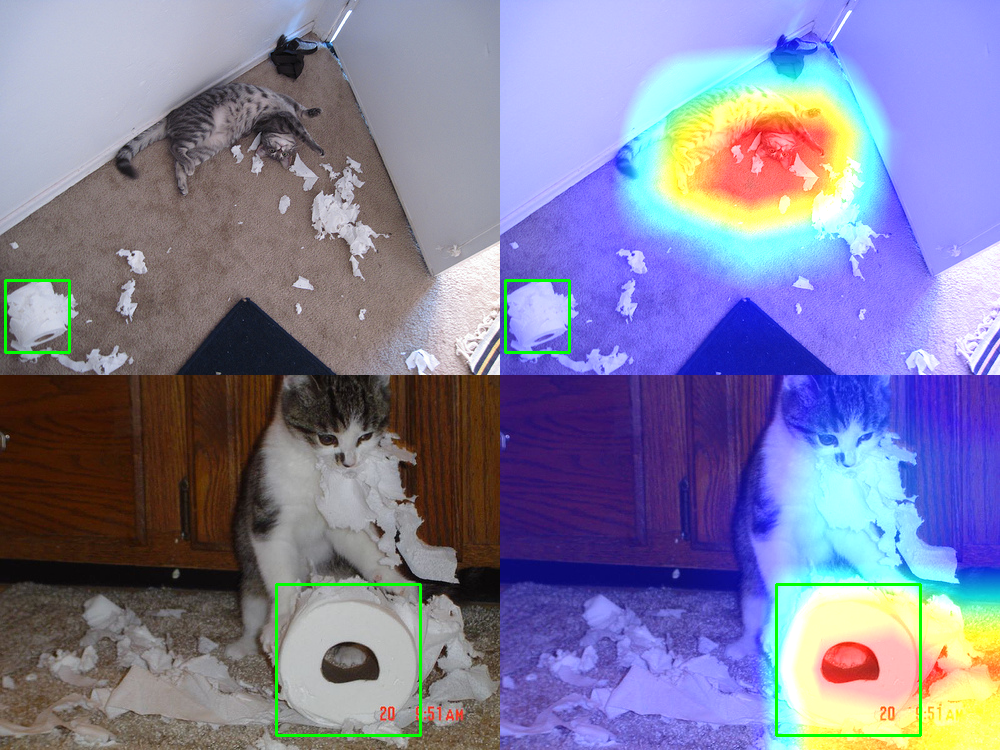
\includegraphics[width=14.2cm]{logo/bad_&_good_CAM_ce.png.png} 
	\caption{Activations par rapport à la classe de vérité terrain (Papier toilette)  : non pertinente (en haut) et pertinente (en bas), avec la boîte de vérité de terain mise en évidence en vert.}
	\label{fig:Exemples d'Activation : Activation Pertinente et Non Pertinente}
\end{figure}
\newpage
\vspace*{0.1\baselineskip}

\hspace{1.6cm}Cette discordance entre la classification et les activations engendre un manque de confiance dans les modèles, car leurs résultats ne sont pas toujours explicables de manière cohérente. En conséquence, il devient crucial d'améliorer l'explicabilité de ces modèles afin que les activations détectées soient davantage pertinentes par rapport à la classification réalisée.
\vspace*{0.5\baselineskip}

\hspace{1.6cm}Le principal objectif de ce stage, comme mentionné dans l'introduction, est donc de proposer des améliorations pour rendre les activations des modèles plus pertinentes et concordantes avec la classification effectuée. Cela permettra de mieux comprendre le processus de décision du modèle et de gagner en confiance quant à l'exactitude de ses prédictions et leur explicabilité.
\vspace*{0.5\baselineskip}

\hspace{1.6cm}Pour atteindre cet objectif, diverses approches peuvent être envisagées. Il est possible d'explorer de nouvelles méthodes d'attribution d'importance aux caractéristiques apprises par le modèle, ou encore d'introduire des mécanismes d'apprentissage supplémentaires visant à renforcer la corrélation entre les activations et la classification. De plus, il peut être intéressant d'investiguer les raisons sous-jacentes des incohérences observées et de proposer des stratégies pour les atténuer.
\newpage

\hspace{1.6cm}Le résultat attendu de ce travail serait donc une meilleure compréhension de la façon dont les modèles de classification prennent leurs décisions, rendant ainsi leurs activations plus fiables et explicables. Ces améliorations pourraient contribuer à accroître l'adoption et l'utilisation de ces modèles dans des domaines critiques tels que la santé, la sécurité ou encore l'automobile autonome, où une interprétabilité fiable est primordiale.

\chapter{État de l'art}

\section{Datasets}
\subsection{Imagenet}

\hspace{1.6cm}ImageNet\cite{ILSVRC15} est une base de données d'images organisée selon la hiérarchie WordNet (actuellement uniquement pour les noms), dans laquelle chaque nœud de la hiérarchie est représenté par des centaines et des milliers d'images. Ce projet a joué un rôle essentiel dans l'avancement de la recherche en vision par ordinateur et en apprentissage profond. Les données sont disponibles gratuitement pour les chercheurs à des fins non commerciales.

\hspace{1.6cm}On a utilisé cette base de données pour 3 raisons : premièrement, parce qu'elle est très grande (plus de 14 millions d'images). Deuxièmement, nous disposons des boîtes de vérité terrain pour des centaines d'images par classe. Et troisièmement, les modèles de classification avec lesquels nous travaillons ont déjà été entraînés sur ImageNet.

\begin{figure}[htbp] 
	\centering
        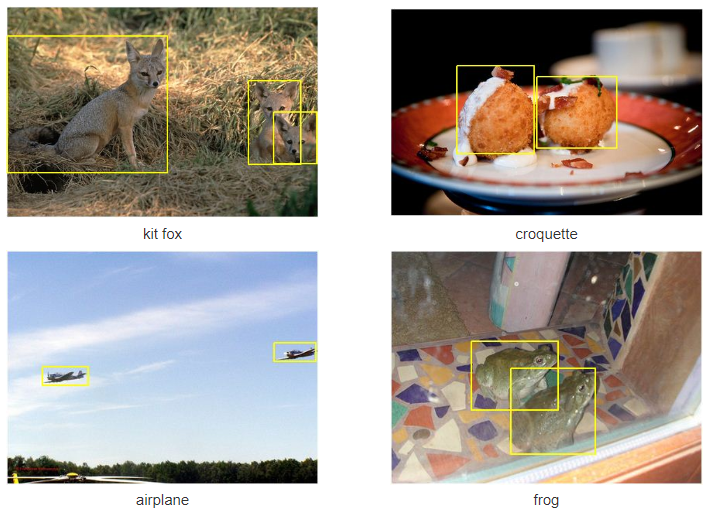
\includegraphics[width=11.3cm]{logo/Imagenet_bb.png} 
	\caption{Exemples d'image provenants d'IMAGENET avec leurs boîtes de vérité terrain}
	\label{fig:Exemples d'image provenants d'IMAGENET avec leurs boîtes de vérité terrain}
\end{figure}

% \subsection{Paludisme (MALARIA)}
% \hspace{1.6cm} L'objectif de ce stage est d'obtenir une classification précise des images de cellules en deux classes : parasitées ou saines, tout en assurant une interprétabilité des résultats de classification. Pour atteindre cet objectif, nous allons utiliser non seulement la base de données IMAGENET, mais également l'ensemble de données sur le paludisme. Ce dernier ensemble contient un total de 27 558 images de cellules, mais nous ne prendrons en compte que les images pour lesquelles nous disposons d'une boîte de vérité de terrain, soit plus de 2800 images, afin de disposer de données annotées pour l'apprentissage du modèle de classification. Ces images proviennent de lames de frottis sanguins minces de cellules segmentées. 
% \vspace*{0.5\baselineskip}
% \begin{figure}[htbp] 
% 	\centering
%         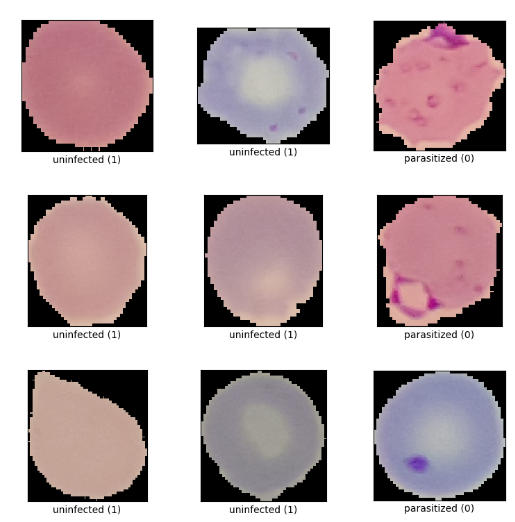
\includegraphics[width=10cm]{logo/Malaria.png} 
% 	\caption{Exemple d'image provenants de la base de données Paludisme}
% 	\label{fig:Exemple d'image provenants de la base de données Paludisme}
% \end{figure}
% }

\section{Modèles}
\hspace{1.6cm}Adam et Wyctor\cite{Adam21,Wyctor22} ont travaillé avec le VGG16\cite{simonyan2015deep}. J'ai choisi le ResNet50V2\cite{he2016identity} car il est plus performant en termes de précision de classification que le VGG16\cite{simonyan2015deep}, tout en occupant moins d'espace mémoire avec moins de paramètres. De plus, le ResNet50V2 nécessite moins de temps par étape d'inférence\cite{KerasDoc}.

\section{Carte d'activation de classe (CAM)}
\hspace{1.6cm}Les CAM (pour Class Activation Maps) sont une technique en vision par ordinateur pour visualiser et comprendre les régions d'intérêt des images utilisées par les réseaux de neurones convolutifs lors de la prise de décision. Cette approche permet de localiser visuellement les zones d'une image qui ont le plus contribué à la classification d'une classe spécifique par le modèle.
\vspace*{0.5\baselineskip}
\begin{figure}[htbp] 
	\centering
        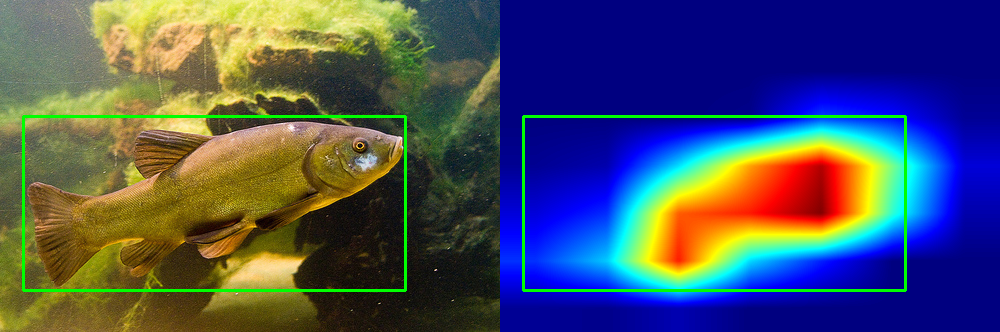
\includegraphics[width=16cm]{logo/CAM.png} 
	\caption{Image d'IMAGENET avec sa boîte de vérité terrain (en vert) et sa CAM par rapport à la classe de vérité terrain (Tanche)}
	\label{fig:Exemples d'image provenants d'IMAGENET avec leurs boîtes de vérité terrain}
\end{figure}

\hspace{1.6cm}Je vais présenter l'évolution des Cartes d'Activation Maximale (CAM) et leur fonctionnement, en mettant en évidence les avancées majeures de la recherche dans ce domaine. Je discuterai des avantages, des limitations et de leur utilisation concrète dans la classification d'images. En outre, je vais explorer la pertinence des CAM dans notre étude et comment elles peuvent améliorer la compréhension et l'interprétation de notre modèle de classification


\subsection{Historique des CAM}

\hspace{1.6cm}Les CAM ont été introduites en 2015 par B. Zhou et al. dans leur article "Learning Deep Features for Discriminative Localization"\cite{Zhou_2016_CVPR}. Depuis lors, les CAM ont suscité un intérêt considérable dans la communauté de la recherche en vision par ordinateur.

\subsection{Fonctionnement des CAM}

\hspace{1.6cm}Les CAM permettent de mettre en évidence les régions d'une image qui contribuent le plus à la classification d'une classe spécifique par le modèle de réseau de neurones convolutifs. Pour cela, la dernière couche convolutive est modifiée de manière à ce que ses activations soient directement liées aux classes d'intérêt. Cela permet de créer une carte de chaleur qui indique les régions d'activation importantes pour chaque classe.
\vspace*{0.5\baselineskip}

\hspace{1.6cm}Pour obtenir les CAM, le réseau est entraîné sur un ensemble de données étiqueté. Une fois l'apprentissage terminé, les activations de la dernière couche convolutive sont pondérées par les poids des neurones dans la couche entièrement connectée correspondant à la classe d'intérêt. Ces activations pondérées sont ensuite agrégées pour créer la carte d'activation pour cette classe spécifique.

\subsection{Grad-Cam et Guided Grad-Cam }

\hspace{1.6cm}Selvaraju et al. \cite{Selvaraju_2017_ICCV} ont introduit la méthode "Grad-CAM" (Gradient-weighted Class Activation Mapping) dans leur article "Grad-CAM: Visual Explanations from Deep Networks via Gradient-based Localization" en 2017. Cette approche a permis d'obtenir des cartes d'activation plus interprétables en utilisant les gradients de la sortie de classe plutôt que les poids des couches.
\vspace*{0.5\baselineskip}

\hspace{1.6cm}À partir d'une image et d'une classe d'intérêt en entrée, ils propagent l'image à travers la partie CNN du modèle, puis effectuent les calculs spécifiques à la tâche pour obtenir un score brut pour la catégorie. Les gradients sont fixés à zéro pour toutes les classes, sauf la classe désirée (tiger cat), qui est fixée à 1. Ce signal est ensuite rétropropagé aux cartes de caractéristiques convolutionnelles rectifiées d'intérêt, qu'ils combinent pour calculer la localisation grossière Grad-CAM (carte de chaleur bleue), qui représente où le modèle doit regarder pour prendre la décision particulière. Enfin, ils multiplient point par point la carte de chaleur avec la propagation guidée pour obtenir des visualisations Guided Grad-CAM, qui sont à la fois haute résolution et spécifiques au concept.
\vspace*{0.5\baselineskip}

\begin{figure}[htbp] 
	\centering
        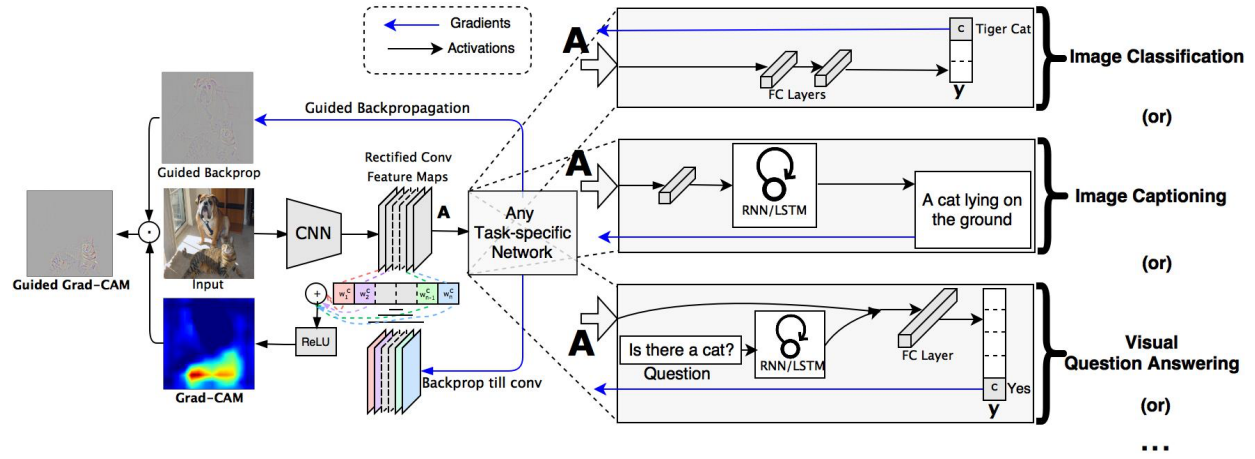
\includegraphics[width=16.5cm]{logo/Grad_cam.png} 
	\caption{Aperçu de Grad-CAM\cite{Selvaraju_2017_ICCV}}
	\label{fig:Aperçu de Grad-CAM}
\end{figure}
\newpage
\subsection{ScoreCam et Faster ScoreCam}
\label{sec:Score}
\hspace{1.6cm}Comme le Grad-CAM, le Score-CAM permet de visualiser les régions importantes des images pour la classification effectuée par le modèle. Cette approche a été introduite par Wang et autres dans leur papier intitulé "Score-Weighted Visual Explanations for Convolutional Neural Networks"\cite{Wang_2020_CVPR_Workshops}.
\vspace*{0.5\baselineskip}

\hspace{1.6cm}Le pipeline proposé du Score-CAM se déroule en deux phases. Dans la première phase, les cartes d'activation sont extraites à partir des couches convolutives du modèle CNN. Chaque carte d'activation agit ensuite comme un masque sur l'image d'origine, et le modèle calcule son score de passage avant (forward-passing score) pour la classe cible. La deuxième phase se répète N fois, où N est le nombre de cartes d'activation. À chaque itération, une nouvelle carte d'activation est utilisée pour mettre en évidence les régions importantes de l'image pour la classe cible. Ainsi, plusieurs cartes d'activation sont obtenues, chacune montrant différentes régions significatives. Enfin, le résultat final est généré en réalisant une combinaison linéaire des poids basés sur les scores obtenus dans la première phase, ainsi que des cartes d'activation elles-mêmes. Cette combinaison permet de mettre en évidence les zones les plus importantes de l'image qui ont contribué à la prédiction du modèle pour la classe d'intérêt.
\vspace*{0.5\baselineskip}

\hspace{1.6cm}Les phases 1 et 2 partagent le même module CNN en tant qu'extracteur de caractéristiques, ce qui rend le processus plus efficace et évite la duplication des calculs. Ainsi, le Score-CAM fournit des explications visuelles pertinentes et compréhensibles pour les décisions prises par le modèle CNN, améliorant ainsi la transparence et la confiance dans ses prédictions.

\begin{figure}[htbp] 
	\centering
        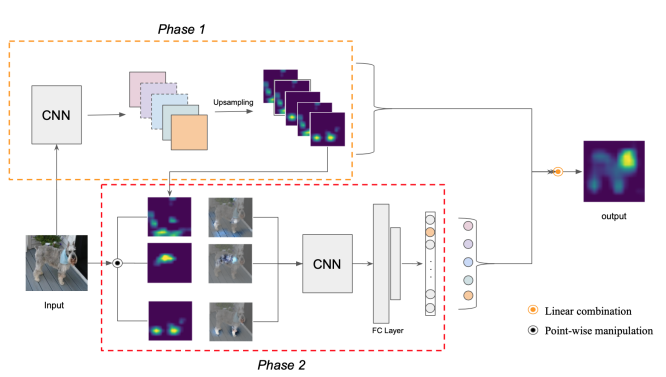
\includegraphics[width=16 cm]{logo/Scorecam.png} 
	\caption{Aperçu de Score-Cam\cite{Wang_2020_CVPR_Workshops}}
	\label{fig:Aperçu de Score-Cam}
\end{figure}
\vspace*{0.5\baselineskip}
\newpage

\hspace{1.6cm}
Le Faster SCORECAM\cite{Wang_2020_CVPR_Workshops} est une amélioration du modèle Score-CAM que nous avons précédemment présenté. Il apporte une optimisation au niveau de la rapidité de calcul par rapport à SCORECAM. En d'autres termes, il est plus efficace en termes de temps d'exécution tout en fournissant des résultats d'interprétation de qualité similaire.
\vspace*{0.1\baselineskip}

\hspace{1.6cm}Cette amélioration est essentielle car elle permet une analyse plus rapide des modèles de vision complexes, ce qui est particulièrement utile lorsque nous traitons de grandes quantités de données ou lorsque nous avons besoin d'obtenir des résultats d'interprétation en temps réel.

\section{Approche Antérieure}
\hspace{1.6cm}Les approches discutées ici ont pour objectif d'améliorer la manière dont un modèle identifie et localise les zones importantes dans une image, plutôt que de se limiter à la simple classification. Cette modification de l'objectif d'optimisation découle de la nécessité de mieux comprendre les décisions du modèle, en particulier dans des domaines où la localisation précise des objets ou des caractéristiques est cruciale, comme la vision par ordinateur.

\hspace{1.6cm}Lorsqu'un modèle est optimisé uniquement pour la classification à l'aide d'une seule fonction de perte (généralement l'entropie croisée), il peut privilégier les caractéristiques globales de l'image au détriment de la localisation précise des objets d'intérêt. Cela peut conduire à des situations où le modèle réussit la classification globale, mais échoue à identifier correctement les zones importantes dans l'image.

\hspace{1.6cm}Au lieu de simplement optimiser la classification, on l'optimise conjointement avec un autre critère, ce qui a conduit à l'introduction du terme HAGTR (ou plus tard le MAGTR) dans la fonction de perte. Cela vise à guider le modèle vers une focalisation accrue sur les zones de l'image correspondant aux emplacements réels des objets d'intérêt, tout en sachant que cela peut potentiellement entraîner une légère diminution de la précision. Cependant, l'objectif est que cette dégradation de la précision soit minime.

\hspace{1.6cm}Le HAGTR, qui correspond à l'activation la plus élevée dans la région de vérité terrain\cite{Wyctor22}. La fonction de perte est alors égale au produit entre l'entropie croisée et (1 - HAGTR). Ils ont utilisé (1 - HAGTR) parce qu'ils minimisent la fonction de perte, donc s'ils veulent maximiser le HAGTR, il faut minimiser -HAGTR. De plus, ils ont ajouté un 1 car le HAGTR est normalisé entre 0 et 1.

\begin{figure}[htbp] 
	\centering
        \adjustimage{width=0.4\textwidth, frame=0.5pt 1.5pt 2pt,center}{logo/Loss_HAGTR.png}
	\caption{Fonction de perte composé de CE et HAGTR}
	\label{fig:Fonction de perte composée de CE et HAGTR}
\end{figure}

\hspace{1.6cm}Le HAGTR a été calculé à partir des CAM (Class Activation Maps) calculées par la méthode GradCam. Cela consiste à prendre la CAM, à l'échantillonner à la taille de l'image d'origine, puis à calculer l'activation la plus élevée dans la région de vérité terrain. Cette approche a été expérimentée sur 2 classes d'IMAGENET (Sac de boxe et épis de maïs), puis sur 14 classes d'IMAGENET. Il est généralement préférable de commencer par une petite base de données pour obtenir rapidement des résultats, car les entraînements prennent beaucoup de temps, et c'est plus facile à gérer et à analyser les résultats.

\hspace{1.6cm}Cependant, les résultats de ces expériences ont abouti à des légères dégradations au niveau de la précision de classification avec une petite amélioration de l'activation dans la région de vérité terrain. Pour cette raison, ils ont essayé une autre approche, en remplaçant le HAGTR par le MAGTR, qui correspond à l'activation moyenne dans la région de vérité terrain. Cette solution n'était pas complète, et c'est à partir de ce point que j'ai continué ces travaux.


\chapter{Approche et travail réalisé}

    \hspace{1.6cm}On a étudié différentes façons d'améliorer à la fois la classification et la localisation de l'activation, dont l'ajout du terme MAGTR à la fonction de perte en combinaison avec l'entropie croisée, on minimise l’entropie croisée tout en maximisant le MAGTR.


\section{Mise en oeuvre}
    La mise en œuvre de ces approches nécessite plusieurs étapes, que je vais détailler ci-dessous :
        \setlist[itemize]{label=\textbullet}

            \begin{itemize}
            \item La préparation  de données : Il convient de noter que les travaux antérieurs sur ce projet portaient sur 2 classes d'ImageNet\cite{ILSVRC15}, Cependant, ma tâche consistait à travailler sur 14 classes d'ImageNet, puis à passer à une échelle plus grande (plus de classes). Pour optimiser les calculs, il était nécessaire de préparer les données avant de démarrer l'entraînement. Cette préparation incluait le chargement des images à partir de notre base de données, leur conversion en tableaux compatibles avec les tenseurs, leur mise à l'échelle et leur normalisation afin d'obtenir une moyenne proche de zéro et une échelle relativement petite. Ces étapes peuvent contribuer à améliorer la stabilité et les performances de l'apprentissage. Ensuite, les étiquettes ont été préparées en les encodant pour qu'elles correspondent à l'entrée du modèle. De plus, un fichier CSV a été préparé pour contenir les coordonnées des boîtes de vérité terrain des images. Enfin, la base de données a été divisée en ensembles d'entraînement, de validation et de test, avec des proportions de 70\%, 15\% et 15 \% respectivement.    
            \item Une fois la préparation des données terminée, la mise en place du modèle à entraîner est intervenue (ResNet50 \cite{he2016identity}). À ce stade, nous avons mis en œuvre la méthode du transfert d'apprentissage, laquelle consiste à utiliser un modèle préalablement entraîné pour identifier des caractéristiques générales de bas niveau présentes dans les données, et ensuite l'adapter pour résoudre une tâche spécifique en ajoutant de nouvelles couches conçues spécifiquement pour cette tâche. Cette approche permet de gagner du temps et d'obtenir de bons résultats, même avec peu de données pour effectuer un entraînement pour une nouvelle tâche. Dans notre cas, nous avons utilisé les couches d'extraction de caractéristiques de ResNet50, préalablement entraîné sur les 1000 classes d'ImageNet \cite{ILSVRC15}, auxquelles nous avons ajouté des couches de classification adaptées au nombre de classes (14).  Cette étape visait à établir un point de référence que nous désignerons comme "époque 0", afin de pouvoir comparer les résultats obtenus avec nos approches ultérieures. Ci-dessous ~\ref{tab:Resnet50_CE}, nous présentons les performances du modèle après cette phase d'entraînement (époque 0), que nous utiliserons comme base de référence pour nos essais ultérieurs.
            
            \renewcommand{\arraystretch}{1.7}
            \begin{table}[ht]
            \centering
            \begin{tabular}{|p{2.7cm}|p{2.7cm}|p{3.2cm}|p{2.7cm}|}
            \hline
            Données & Précision (\%) & Entropie-croisée & MAGTR  \\
           
            \hline
            Validation & 95.84 & 0.1605 & 0.3648  \\
            \hline
            \end{tabular}
            \caption{Tableau de référence (époque 0)}
            \label{tab:Resnet50_CE}
            \end{table}
            
            \item Entraînement multitâches : Suite à la préparation des données et à la mise en place du modèle, une boucle d'apprentissage personnalisée a été élaborée en utilisant TensorFlow\cite{tensorflow2015-whitepaper} et Keras\cite{KerasDoc}. Cette approche sur mesure implique l'utilisation de l'objet "GradientTape" pour enregistrer les opérations effectuées pendant la propagation avant (forward pass) du modèle. À l'intérieur de cette boucle, les prédictions sont calculées, la perte est évaluée en utilisant une fonction de perte définie, et les gradients sont calculés par rapport aux paramètres du modèle. Ces gradients sont ensuite utilisés pour mettre à jour les poids du modèle via un optimiseur sélectionné. Cette boucle est répétée pour chaque lot d'entraînement, permettant ainsi un ajustement progressif des paramètres du modèle et l'amélioration de ses performances sur la tâche donnée.
            \item Ajustement des hyperparamètres : L'ajustement des hyperparamètres consiste à régler des valeurs clés qui ne sont pas directement apprises par le modèle, telles que les taux d'apprentissage et la taille des lots d'entraînement, entre autres. L'objectif est d'optimiser les performances du modèle sur les données d'entrainement et de validation en expérimentant différentes combinaisons de valeurs. Cette étape nécessite généralement une approche itérative, où les performances du modèle sont évaluées sur un ensemble de validation. L'ajustement des hyperparamètres joue un rôle crucial dans l'obtention de modèles d'apprentissage automatique performants et généralisables, adaptés aux spécificités de chaque tâche
            \item L'évaluation : L'évaluation du modèle consiste à mesurer ses performances et sa capacité à effectuer des prédictions précises sur de nouvelles données. Cela implique de tester le modèle sur un ensemble de données distinct (ensemble de test ou de validation) qui n'a pas été utilisé pendant l'entraînement. Les métriques d'évaluation, telles que la précision, l'exactitude, le rappel, etc., permettent de quantifier la qualité des prédictions du modèle. L'évaluation est essentielle pour déterminer si le modèle généralise bien au-delà des données d'entraînement et pour identifier d'éventuelles lacunes ou erreurs à corriger. Nous avons utilisé la précision et le terme MAGTR pour évaluer la qualité de la précision et de l'activation, respectivement.
            \end{itemize}
\hspace{1.6cm}Nous présenterons les résultats des approches que nous avons testées. Chacune de ces expériences a contribué à approfondir notre compréhension du problème et à orienter nos efforts vers des stratégies plus prometteuses, comme le démontrera la discussion à venir.

\section{Essais et Résultats}
\subsection{Essai 1 : Produit}
La fonction de perte est le produit de l'entropie croisée par (1-MAGTR).
    \begin{figure}[htbp] 
	\centering
        \adjustimage{width=0.5\textwidth, frame=0.5pt 1.5pt 2pt,center}{logo/prod_loss.png}
	\caption{Fonction de perte composé de CE multipliée par MAGTR}
	\label{fig:Fonction de perte composé de CE multipliée par MAGTR}
    \end{figure}


\hspace{1.6cm}Il est important de noter que l'ajustement des hyperparamètres lors de l'entraînement prend beaucoup de temps, pouvant s'étendre sur plusieurs jours voire des semaines. Dans le cadre de notre expérience, un autre hyperparamètre crucial est le nombre de canaux N\_max (ou max\_N), qui est un paramètre de Faster-Scorecam, comme expliqué dans le chapitre État de l'art \autoref{sec:Score}. Ce paramètre correspond au nombre maximal de canaux à prendre en compte pour calculer la carte d'activation. Son utilisation accélère significativement l'entraînement et évite les contraintes liées à la mémoire. Par conséquent, je ne présenterai ici que les expériences ayant donné les meilleurs résultats en termes d'hyperparamètres.
\vspace*{0.5\baselineskip}

\hspace{1.6cm}En ce qui concerne le produit, nous avons initialement essayé d'ajuster la taille des lots d'entraînement. Cependant, le code n'était pas compatible avec différentes tailles de lots, car il ne traitait qu'une seule image par lot. Pour résoudre ce problème, nous avons entrepris des modifications substantielles dans le code. Nous avons revu et adapté toutes les fonctions utilisées dans la boucle d'entraînement afin qu'elles puissent traiter efficacement les images par lot de tailles variables. Ces ajustements nous ont permis d'assurer la compatibilité du code avec différentes tailles de lots, améliorant ainsi la flexibilité et les performances globales du système. Ensuite, nous avons cherché à déterminer la meilleure valeur pour N\_max. Malheureusement, en raison des contraintes de mémoire, nous n'avons pas pu explorer des valeurs étendues de N\_max (au-delà de 50 canaux) ni utiliser des tailles de lots importantes (au-delà de 6 images) dans le cadre de cette approche. Cependant, j'ai réussi à accroître la taille du lot en utilisant une technique d'accumulation de gradient, ce qui a permis de contourner ces limitations. Cette méthode fonctionne en divisant un lot en sous-lots plus petits, calculant les gradients pour chaque sous-lot, puis en accumulant ces gradients avant de mettre à jour les poids du modèle. Cela permet d'exploiter des lots plus grands sans surcharger la mémoire, améliorant ainsi les performances globales du processus d'apprentissage.

\vspace*{0.5\baselineskip}

\hspace{1.6cm}Cette expérience a a permis de corriger de nombreuses erreurs présentes dans le programme, que ce soit lors de la préparation des données, de la boucle d'entraînement ou de l'évaluation.

Voici le meilleur résultat que nous avons obtenu pour le produit : 

\begin{figure}[htbp] 
	\centering
        \adjustimage{width=1\textwidth, frame=0.5pt 1.5pt 2pt,center}{logo/prod_train_curves.png}
	\caption{Courbes d'apprentissage avec la fonction de perte "produit" \ref{fig:Fonction de perte composé de CE multipliée par MAGTR}}
	\label{fig:Courbes d'apprentissage avec la fonction de perte "produit"}
\end{figure}

\hspace{1.6cm}Pour toutes les expériences on analyse les 4 courbes ci-dessus, la precision, le MAGTR qu'on maximise, l'entropie croisée et la fonction perte, pour savoir la qualité de la précision, la qualité de l'activation et comment le model apprend au cours des époques. 

\hspace{1.6cm}On observe sur la courbe du MAGTR une diminution, tout comme une dégradation significative de la précision. L'analyse des courbes issues de cette expérience révèle une particularité intrigante : les valeurs de perte constatées sur les données de validation se révèlent en effet inférieures à celles enregistrées lors de l'entraînement, comme présenté dans la figure ~\ref{fig:Courbes d'apprentissage avec la fonction de perte "produit"}. Ces constatations indiquent la nécessité d'envisager un changement d'approche.

\newpage
\subsection{Essai 2 : Division}
\hspace{1.6cm}Après l'essai 1 nous avons changé le produit par la division.Par conséquent, la différence réside dans la formule de la fonction de perte,où nous avons exploré la diviser l'entropie croisée par le MAGTR. On a suivi les mêmes étapes de l'expérience précedente, pour ajuster les hyperparamètres. 

\begin{figure}[htbp] 
	\centering
        \adjustimage{width=0.33\textwidth, frame=0.5pt 1.5pt 2pt,center}{logo/div_loss.png}
	\caption{Fonction de perte composé de CE divisée par MAGTR}
	\label{fig:Fonction de perte composé de CE divisée par MAGTR}
\end{figure}

Voici le résultat le plus optimal que nous avons pu obtenir pour la division :
\begin{figure}[htbp] 
	\centering
        \adjustimage{width=1\textwidth, frame=0.5pt 1.5pt 2pt,center}{logo/div_train_curves.png}
	\caption{Courbes d'apprentissage avec la fonction de perte "division" \ref{fig:Fonction de perte composé de CE divisée par MAGTR}}
	\label{fig:Courbes d'apprentissage de l'expérience division}
\end{figure}

\hspace{1.6cm}Les courbes d'apprentissage de cette expérience mettent en évidence une mauvaise précision et un MAGTR faible. Les résultats demeurent globalement insatisfaisants. Cette convergence souligne la persistance des problèmes identifiés précédemment, nécessitant une réévaluation attentive de nos approches et paramètres expérimentaux.


\subsection{Essai 3 : Somme pondérée }
\hspace{1.6cm}Après tous ces tests, nous avons découvert plusieurs travaux sur internet qui utilisaient la somme pondérée pour un entraînement multitâche, lorsqu'un modèle doit apprendre deux tâches ou plus simultanément, dont un article \cite{Kendall_2018_CVPR}. Nous avons suivi cette approche en effectuant la somme pondérée des deux termes que nous souhaitons optimiser, à savoir l'entropie croisée et le MAGTR.  

    \begin{figure}[htbp] 
	\centering
        \adjustimage{width=0.5\textwidth, frame=0.5pt 1.5pt 2pt,center}{logo/sum_loss.png}
	\caption{Fonction de perte de la somme pondérée de CE et MAGTR}
	\label{fig:Fonction de perte de la somme pndérée de CE et MAGTR}
    \end{figure}


\hspace{1.6cm}Lors de la conduite de cette expérience, nous avons suivi les mêmes étapes méthodologiques que celles précédemment entreprises pour ajuster les hyperparamètres du modèle. Cependant, pour surmonter des instabilités et converger vers un optimum, il a fallu accorder une attention particulière à deux hyperparamètres essentiels : la taille des lots (batch size) et le taux d'apprentissage (learning rate). 
    \vspace*{0.5\baselineskip}

\hspace{1.6cm}Étant limités par la capacité de mémoire RAM, nous avons initialement restreint le nombre d'images par lot, ce qui a eu un impact négatif sur la convergence du modèle. Pour résoudre ce problème, nous avons adopté une stratégie de gradient accumulatif, accumulant les gradients sur plusieurs lots avant la mise à jour des poids du modèle. De plus, nous avons réajusté le taux d'apprentissage pour compenser les changements introduits par la modification de la taille des lots. Ces ajustements conjoints ont permis de rétablir la convergence de l'apprentissage et d'améliorer les performances du modèle, 
    \vspace*{0.5\baselineskip}

\hspace{1.6cm}Deux nouveaux hyperparamètres ont été pris en considération exclusivement pour cette expérimentation, à savoir les coefficients (k1 et k2) de la somme pondérée\ref{fig:Fonction de perte de la somme pndérée de CE et MAGTR}.
Les résultats les plus optimaux que nous avons obtenus pour ces expériences sont les suivants :

    \begin{figure}[htbp] 
	\centering
        \adjustimage{width=0.9\textwidth, frame=0.5pt 1.5pt 2pt,center}{logo/sum_train_curves.png}
	\caption{Courbes d'apprentissage avec la fonction de perte "somme-pondérée"\ref{fig:Fonction de perte de la somme pndérée de CE et MAGTR}}
	\label{fig:Courbes d'apprentissage de l'expérience "somme-pondérée"}
    \end{figure}
\newpage
\hspace{1.6cm}Les courbes de la figure \ref{fig:Courbes d'apprentissage de l'expérience "somme-pondérée"} illustrent une légère dégradation de la précision, ainsi qu'une nette amélioration du MAGTR. Toutefois, afin de déterminer si cette augmentation du MAGTR après l'entraînement correspond à une activation significative ou non, il est nécessaire de générer les cartes d'activation pour les images correctement classées avant l'entraînement (époque 0) et après l'entraînement (en sélectionnant la meilleure époque, soit l'époque 18 selon les courbes d'apprentissage \ref{fig:Courbes d'apprentissage de l'expérience "somme-pondérée"}).

Ainsi, nous recherchons ces images dans des fichiers CSV générés après l'entraînement, contenant les valeurs du MAGTR. Nous ciblons spécifiquement les images qui ont des valeurs faibles du MAGTR, et ayant été correctement classées par les modèles après les deux époques.

Ci-dessous, des exemples de ces images accompagnées de leurs activations correspondantes :
    \begin{figure}[htbp] 
	\centering
        \adjustimage{width=0.9\textwidth, frame=0.5pt 1.5pt 1pt,center}{logo/good_and_bad_cams.png}
	\caption{Cartes d'activation par rapport à la classe de vérité terrain (1ère image : Noeud papillon, 2ème image : Noeud papillon, 3ème image : blouse de laboratoire, 4ème image : MAmba vert, 5ème image : Grand requin blanc, 6ème image : Rainette) pour les images correctement classées par les modèles après les époques 0 et 18, tout en présentant un MAGTR faible. À gauche, les images originales ; au milieu, les CAMs de l'époque 0 ; à droite, les CAMs de l'époque 18.}
	\label{fig:CAMs de CE & Sum"}
    \end{figure}
\newpage
Les observations que nous pouvons tirer de ces CAMs indiquent que le MAGTR modifie peu la localisation des activations, en particulier les mauvaises localisations, mais il étend leur étendue. Cependant, la précision n'a pas subi une dégradation remarquable, on peut mieux voir cela sur les matrices de confusion de l'époque 0 et 18 des données de test.
    \begin{figure}[htbp] 
	\centering
        \adjustimage{width=1\textwidth, frame=0.5pt 1.5pt 1pt,center}{logo/Conf_mat0.png}
	\caption{Matrice de confusion du modèle Resnet50 \cite{he2016identity} entraîné sur l'entropie croisée pour 14 classes d'ImageNet (époque 0 de l'essai : somme pondérée \ref{fig:Courbes d'apprentissage de l'expérience "somme-pondérée"}).}
	\label{fig:Matrice de confusion ep0"}
    \end{figure}
    
    \begin{figure}[htbp] 
	\centering
        \adjustimage{width=1\textwidth, frame=0.5pt 1.5pt 1pt,center}{logo/Conf_mat18.png}
	\caption{Matrice de confusion du modèle Resnet50 \cite{he2016identity} entraîné sur la somme pondérée de l'entropie croisée et le MAGTR pour 14 classes d'ImageNet (époque 14 de l'essai : somme pondérée \ref{fig:Courbes d'apprentissage de l'expérience "somme-pondérée"}).}
	\label{fig:Matrice de confusion ep18"}
    \end{figure}

\newpage
Les conclusions que nous pouvons tirer de cet essai (somme pondérée) est la précision est peu affectée par le compromis (optimisation multi-tâches : la CE et le MAGTR). Toutefois, cela ne répond toujours pas à notre objectif d'obtenir des localisations précises des activations dans le cas de prédictions correctes.


\chapter{Difficultés Rencontrées}
\section{Code existant peu lisible et non optimisé}
    \hspace{1.6cm}Au début de mon stage, j'ai été confronté à un code implémenté par de précédents stagiaires Adam Aalah\cite{Adam21} et Wyctor Fogos da Rocha \cite{Wyctor22} qui présentait des problèmes de lisibilité et de structuration. Cela rendait ma compréhension du code difficile et m'a causé des difficultés pour effectuer des modifications et des améliorations. En particulier, j'ai simplifié le code de W. Fogos da Rochas qui effectuait un calcul explicite des gradients en utilisant partout des tenseurs gérés par le mécanisme de différentiation automatique de Tensorflow. De plus, j'ai dû faire face à des incompatibilités entre les versions des bibliothèques et frameworks utilisés, comme TENSORFLOW\cite{tensorflow2015-whitepaper} et CUDA\cite{nvidia_cuda_guide}, ce qui compliquait la tâche de faire fonctionner le code correctement.
\section{Bugs et limitations de mémoire}    
    \hspace{1.6cm}Après avoir acquis une meilleure compréhension de la problématique et des approches à suivre, j'ai dû résoudre des bugs présents dans le code existant. Ces erreurs ont nécessité des efforts supplémentaires pour les identifier et les corriger. Par ailleurs, en raison de limitations de mémoire, j'ai dû optimiser le code pour résoudre les problèmes de limitation et garantir le bon fonctionnement des calculs.
\section{Migration vers GOOGLE COLAB et limitations associées}
    \hspace{1.6cm}Ensuite on a essayé de changer la plateforme en utilisant GOOGLE COLAB\cite{google_colab} au lieu de Jupyter\cite{jupyter} dans la machine locale. L'exécution était plus rapide par contre il y avait d'autres limitations l’espace mémoire de stockage et la session d'exécution s'arrête après 12 heures, de plus les ressources ne sont pas toujours disponibles surtout le GPU (qui est nécessaire pour nos calculs).

\section{Transition vers VSCODE avec des scripts PYTHON}    
    \hspace{1.6cm}Après avoir surmonté ces limitations j'ai continué le travail sur Jupyter pour quelque semaines, avant de passer à VSCODE\cite{vscode} en utilisant des scripts PYTHON plutôt qu'un NOTEBOOK Jupyter pour plusieurs avantages :
    
  
    \setlist[itemize]{label=\textbullet}
    
        \begin{itemize}
            \item Les scripts Python peuvent être intégrés dans des applications ou des projets plus vastes, ce qui permet une utilisation plus souple et une meilleure maintenance du code.
            \item Les scripts Python peuvent être facilement automatisés pour s'exécuter à intervalles réguliers ou en réponse à des événements spécifiques. De plus, en organisant le code en fonctions et modules, vous pouvez le réutiliser plus facilement dans d'autres projets.
            \item Dans certaines situations, exécuter un script Python peut être plus rapide qu'un notebook Jupyter, car les cellules du notebook ont une surcharge supplémentaire en raison de leur nature interactive.
            \item Lorsque vous exécutez un script Python, les variables sont encapsulées dans l'espace de noms du script. Cela réduit le risque de pollution des variables globales, ce qui peut être plus problématique dans un notebook Jupyter où les cellules partagent un espace de noms global.
        \end{itemize}

\section{Migration vers la plateforme de calcul départementale Vulkan }   
    \hspace{1.6cm}J'ai rencontré des difficultés lors de mes tentatives pour exécuter les scripts sur ma machine locale. Les problèmes de compatibilité entre TENSORFLOW et CUDA sous Windows se sont révélés complexes à résoudre. Cependant, une solution alternative s'est présentée sous la forme de la plateforme de calcul départementale, Vulkan. Avec l'aide de collègues expérimentés dans la gestion de cette plateforme, nous avons mis en place un environnement virtuel minutieusement configuré. Cet environnement incluait toutes les bibliothèques nécessaires pour exécuter sans encombre mes scripts.
    
    \hspace{1.6cm}La réussite de cette solution a été déterminante. Les scripts ont pu être exécutés de manière fluide et performante au sein de cet environnement Vulkan. Devant cette efficacité, j'ai poursuivi mon travail exclusivement sur la plateforme de calcul de l'école, sans résoudre les problèmes de ma machine locale jusqu'à ce que j'avance davantage dans mes travaux. Cette décision m'a permis de continuer à progresser efficacement dans mes projets sans être entravé par les difficultés de compatibilité que j'avais rencontrées initialement sur ma machine locale.

    Le nœud de calcul attribué pour mes travaux était spécifiquement configuré comme suit :
    \begin{itemize}
        \item Mémoire RAM : 26 Go
        \item Système d'Exploitation : Linux
        \item Carte Graphique : NVIDIA GeForce RTX 1080Ti (Capacité de GPU : 11 Go)
    \end{itemize}
    Cette configuration a été essentielle pour maximiser les performances de calcul et de traitement graphique
    \vspace*{0.5\baselineskip}
En conclusion, ces difficultés rencontrées lors de mon stage ont été essentielles pour
mon apprentissage, m’aidant à mieux comprendre les enjeux du projet et à développer
mes compétences professionnelles tout au long du processus d’adaptation
\chapter{Conclusion}
\hspace{1.6cm}En conclusion, cette mission au sein du département ARTEMIS de l'école Telecom SudParis a été une opportunité enrichissante d'explorer le domaine de la vision par ordinateur et d'étudier les cartes de saillance pour améliorer la fiabilité des décisions de classification obtenues par les réseaux convolutifs. Malgré des obstacles tels que le code peu lisible, les limitations de mémoire et les ajustements aux environnements GOOGLE COLAB \cite{google_colab}, VSCODE \cite{vscode} et la plateforme de calcul départementale Vulkan, nos efforts ont abouti à l'élaboration d'une approche prometteuse basée sur l'intégration des cartes de saillance dans le processus d'apprentissage des réseaux convolutifs.
\vspace*{0.5\baselineskip}

\hspace{1.6cm}Les résultats des essais menés ont été significatifs, en particulier dans l'expérimentation relative à la somme pondérée, qui a renforcé notre confiance en l'efficacité de notre méthode pour améliorer les performances de classification. Cependant, l'essai de la somme pondérée demeure encore insuffisant, soulignant la nécessité de rechercher des améliorations, comme suggéré dans les perspectives. À cet égard, notre travail futur consistera à explorer davantage cette voie dans le cadre de cette mission.
\vspace*{0.5\baselineskip}

\hspace{1.6cm}En somme, cette mission a été une expérience marquante qui témoigne de notre engagement envers le domaine de la vision par ordinateur, mettant en avant notre désir de contribuer à l'amélioration constante des méthodes et solutions.

 

\chapter{Perspectives}

Les travaux à effectuer pour le reste du stage, sur une période de six semaines, comprennent :
\begin{itemize}
    \item Intégration du terme MANGTR : Une avenue prometteuse serait l'intégration du terme MANGTR (Mean Activation Not Ground Truth Region) à la fonction de perte de l'essai Somme pondérée. Cette démarche viserait à pénaliser les activations en dehors de la région de vérité terrain, potentiellement améliorant ainsi la performance globale de la méthode en réduisant les erreurs de classification.

    \item Tests avec Fast ScoreCam \cite{li2023fimf} et GradCAM\cite{Selvaraju_2017_ICCV} : Il serait opportun de répéter les tests en utilisant les méthodes alternatives Fast ScoreCam et GradCAM. Cela permettrait une comparaison approfondie des performances des différentes approches de génération de cartes de saillance, en prenant en compte le coût computationnel élevé associé à ScoreCAM \cite{Wang_2020_CVPR_Workshops}.

    \item Évaluation étendue : Étendre l'évaluation de la méthode choisie serait une étape cruciale. Actuellement, basée sur des essais portant sur 14 classes, une évaluation à plus grande échelle avec environ 200 classes de la base de données ImageNet fournirait des conclusions plus solides et une meilleure compréhension des performances.
\end{itemize}

Ces perspectives rapprochent notre travail des objectifs visés et reflètent notre dévouement à l'amélioration continue des méthodes de vision par ordinateur. En mettant l'accent sur l'optimisation du code, la gestion des contraintes matérielles et l'exploration de nouvelles avenues, nous visons à consolider notre contribution à ce domaine en constante évolution.

\printbibliography
\chapter{Annexes}
\section{Travaux Additionnels Post-Soutenance}
\subsection{Intégration du MANGTR}

\hspace{1.6cm}Comme mentionné dans les perspectives, nous avons essayé d'intégrer un nouveau terme dans la fonction de perte, le MANGTR (activation moyenne hors de la région de vérité de terrain). Pour ce faire, nous avons suivi les mêmes étapes que lors des expériences précédentes pour ajuster les hyperparamètres et les poids de chacun des termes (CE, MAGTR et MANGTR) de la fonction de perte.

    
    \begin{figure}[htbp] 
	\centering
        \adjustimage{width=0.6\textwidth, frame=0.5pt 1.5pt 2pt,center}{logo/sum_loss_mangtr.png}
	\caption{Fonction de perte de la somme pondérée de CE, MAGTR et MANGTR}
	\label{fig:Fonction de perte de la somme pndérée de CE, MAGTR et MANGTR}
    \end{figure}
    
\hspace{1.6cm}Lors de ces expériences, nous avons remarqué que lorsque nous attribuons un poids élevé au terme MAGTR, le MANGTR ne s'améliore pas suffisamment, comme illustré dans l'exemple ci-dessous où nous avons attribué un poids élevé. Cependant, lorsque nous attribuons un faible poids au MAGTR, le MAGTR montre une dégradation, tandis que le MANGTR n'enregistre pas d'amélioration significative, comme le démontre l'exemple ci-dessous où nous avons attribué un poids faible.

    \begin{figure}[htbp] 
	\centering
        \adjustimage{width=0.95\textwidth, frame=0.5pt 1.5pt 2pt,center}{logo/sum_train_curves_man33.png}
	\caption{Courbes d'apprentissage avec la fonction de perte "somme-pondérée (33,33,34)" \ref{fig:Fonction de perte de la somme pndérée de CE, MAGTR et MANGTR}}
	\label{fig:Courbes d'apprentissage de l'expérience "somme-pondérée mangtr333"}
    \end{figure}

    \begin{figure}[htbp] 
	\centering
        \adjustimage{width=0.95\textwidth, frame=0.5pt 1.5pt 2pt,center}{logo/sum_train_curves_man55.png}
	\caption{Courbes d'apprentissage avec la fonction de perte "somme-pondérée (5,5,90)" \ref{fig:Fonction de perte de la somme pndérée de CE, MAGTR et MANGTR}}
	\label{fig:Courbes d'apprentissage de l'expérience "somme-pondérée mangtr5595"}
    \end{figure}
\newpage
\hspace{1.6cm}Donc, un poids faible sur le MAGTR avec un poids fort sur le MANGTR n'empêche pas la dégradation du MAGTR, en revanche, il dégrade bien le MANGTR. C'est pourquoi nous avons essayé d'attribuer un poids nul au MAGTR et un poids fort sur le MANGTR, comme le démontrent les courbes d'apprentissage ci-dessous :
    \begin{figure}[htbp] 
	\centering
        \adjustimage{width=0.95\textwidth, frame=0.5pt 1.5pt 2pt,center}{logo/sum_train_curves_man50.png}
	\caption{Courbes d'apprentissage avec la fonction de perte "somme-pondérée (5,0,95)" \ref{fig:Fonction de perte de la somme pndérée de CE, MAGTR et MANGTR}}
	\label{fig:Courbes d'apprentissage de l'expérience "somme-pondérée mangtr5095"}
    \end{figure}



\hspace{1.6cm}Comme on a fait avec les experiences précedentes, aprés l'analyse des courbes d'apprentissage on passe au analyse des cartes d'activation, sauf ici on a changé la méthode du choix des images. On a pris les images qui ont été correctement classées à l'époque 0 et sont devenues mal classées, ainsi que les images qui ont été mal classées et sont devenues correctement classées. 

\hspace{1.6cm}Ci-dessous, des exemples (de l'experience de la figure \ref{fig:Courbes d'apprentissage de l'expérience "somme-pondérée mangtr5095"} de ces images accompagnées de leurs activations correspondantes :









\chapter*{Abstract}
\section*{Résumé}
\hspace{1.6cm}Ce rapport de stage témoigne de notre engagement au sein du département ARTEMIS de l'école Telecom SudParis, où nous avons entrepris une mission passionnante visant à améliorer la fiabilité des classifications obtenues par les réseaux convolutifs grâce à l'exploration des cartes de saillance dans le domaine de la vision par ordinateur. Notre démarche a été axée sur l'intégration de l'activation des cartes de saillance dans le processus d'apprentissage, en utilisant des ensembles de données tels qu'ImageNet. Ce travail s'inscrit dans la continuité des recherches entreprises par les précédents stagiaires, Adam Allah et Wyctor Fogos da Rochas. Ce rapport détaille nos efforts, des étapes initiales de collecte des données à l'évaluation approfondie des performances de nos approches.

\section*{Mots-clés}
Vision par ordinateur, Réseaux de neurones convolutifs, Classification d'images, Carte d'activation de classe, Explicabilité du modèle, ScoreCam.


\section*{Summary}
\hspace{1.6cm}This internship report reflects our commitment within the ARTEMIS department at Telecom SudParis, where we embarked on an exciting mission to enhance the reliability of classifications obtained through convolutional networks by exploring saliency maps in the field of computer vision. Our approach focused on integrating saliency map activations into the learning process, utilizing datasets such as ImageNet. This work builds upon the research pursued by previous interns, Adam Allah and Wyctor Fogos da Rochas. This report elaborates on our endeavors, from the initial data collection steps to the comprehensive evaluation of our approaches' performances.

\section*{Keywords}
Computer Vision, Convolutional Neural Networks, Image Classification, Class Activation Mapping, Model Explainability, ScoreCam}
\end{document}
